%\documentclass[mathserif]{beamer}
\documentclass[handout]{beamer}
%\usetheme{Goettingen}
\usetheme{Warsaw}
%\usetheme{Singapore}
%\usetheme{Frankfurt}
%\usetheme{Copenhagen}
%\usetheme{Szeged}
%\usetheme{Montpellier}
%\usetheme{CambridgeUS}
%\usecolortheme{}
%\setbeamercovered{transparent}
\usepackage[english, activeacute]{babel}
\usepackage[utf8]{inputenc}
\usepackage{amsmath, amssymb}
\usepackage{dsfont}
\usepackage{graphics}
\usepackage{cases}
\usepackage{graphicx}
\usepackage{pgf}
\usepackage{epsfig}
\usepackage{amssymb}
\usepackage{multirow}	
\usepackage{amstext}
\usepackage[ruled,vlined,lined]{algorithm2e}
\usepackage{amsmath}
\usepackage{epic}
\usepackage{epsfig}
\usepackage{fontenc}
\usepackage{framed,color}
\usepackage{palatino, url, multicol}
\usepackage{listings}
%\algsetup{indent=2em}


\vspace{-0.5cm}
\title{Model Evaluation and Information Criteria}
\vspace{-0.5cm}
\author[Felipe Bravo Márquez]{\footnotesize
%\author{\footnotesize  
 \textcolor[rgb]{0.00,0.00,1.00}{Felipe José Bravo Márquez}} 
\date{ \today }




\begin{document}
\begin{frame}
\titlepage


\end{frame}


%%%%%%%%%%%%%%%%%%%%%%%%%%%


\begin{frame}{Model Evaluation and Information Criteria}
\scriptsize{
\begin{itemize}
\item In this class we will introduce various concepts for evaluating statistical models.

\item According to \cite{mcelreath2020statistical}, there are two fundamental kinds of statistical error:

\begin{itemize}\scriptsize{
 \item \textbf{Overfitting}: models that learn  too much from the data leading to poor prediction.
\item \textbf{Underfitting}: moderls that learn too little from the data, which also leads to poor prediction.}
\end{itemize}

\item We will study two common families of approaches to tackle these problems.


\begin{itemize}\scriptsize{
 \item \textbf{Regularization}: a mechanism to tell our models not to get too excited by the data.
\item \textbf{Information criteria}: a scoring device to estimate predictive accuracy of our models.}
\end{itemize}

\item In order to introduce information criteria, this class must also introduce some concepts of \textbf{information theory}.

 
\end{itemize}



} 

\end{frame}



\begin{frame}{The problem with parameters}
\scriptsize{

\begin{itemize}
\item In the class of linear regression we learned that including more attributes can lead to a more accurate model.

\item However, we also learned that adding more variables almost always improves the fit of the model to the data, as measured by the coefficient of determination $R^2$. 
\item This is true even when the variables we  add to a model have no relation to the outcome. 

\item So it's no good to choose among models using only fit to the data.






\end{itemize}


} 
\end{frame}

\begin{frame}{The problem with parameters}
\scriptsize{

\begin{itemize}

\item While more complex models fit the data better, they often predict new data worse.

\item This means that a complex model will be very sensitive to the exact sample used to fit it.

\item This will lead to potentially large mistakes when future data is not exactly like the past data.

\item But simple models, with too few parameters, tend instead to underfit, systematically over-predicting or under-predicting the data.

\item Regardless of how well future data resemble past data. 
\item So we can't always favor either simple models or complex models.

\item Let’s examine both of these issues in the context of a simple data example.

\end{itemize}


} 
\end{frame}


\begin{frame}[fragile]{The problem with parameters}
\scriptsize{

\begin{itemize}

\item We are going to create a data.frame containing  average brain volumes and body masses for seven hominin species.

\begin{verbatim}
sppnames <- c( "afarensis","africanus","habilis",
               "boisei", "rudolfensis","ergaster",
               "sapiens")
brainvolcc <- c( 438 , 452 , 612, 521, 752, 871, 
                 1350 )
masskg <- c( 37.0 , 35.5 , 34.5 , 41.5 , 55.5 , 
             61.0 , 53.5 )
d <- data.frame( species=sppnames , brain=brainvolcc,
                 mass=masskg ) 
\end{verbatim}

\item It's not unusual for data like this to be highly correlated.
\item Brain size is correlated with body size, across
species. 

\end{itemize}


} 
\end{frame}


\begin{frame}[fragile]{The problem with parameters}
\scriptsize{

\begin{figure}[h!]
	\centering
	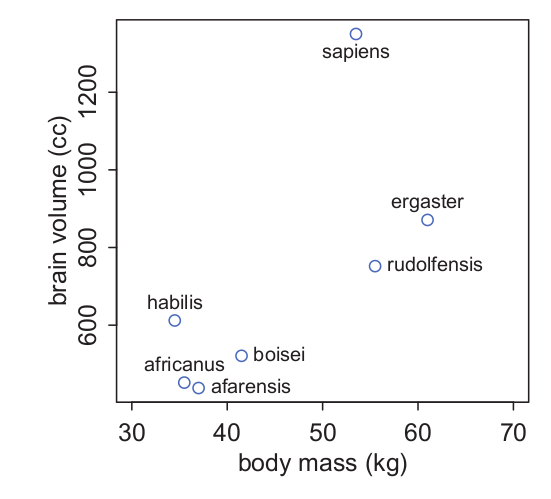
\includegraphics[scale=0.41]{pics/hominin.png}
\end{figure}


} 
\end{frame}


\begin{frame}[fragile]{The problem with parameters}
\scriptsize{

\begin{itemize}

\item We will model brain size as a function of body size.

\item We will fit a series of increasingly complex model families and see which function fits the data best.

\item Each of these models will just be a polynomial of higher degree.

\begin{verbatim}
reg.ev.1 <- lm( brain ~ mass , data=d )
reg.ev.2 <- lm( brain ~ mass + I(mass^2)
                , data=d )
reg.ev.3 <- lm( brain ~ mass + I(mass^2)
                + I(mass^3),data=d )
reg.ev.4 <- lm( brain ~ mass + I(mass^2)
                + I(mass^3) + I(mass^4),data=d )
reg.ev.5 <- lm( brain ~ mass + I(mass^2)
                + I(mass^3) + I(mass^4)
                + I(mass^5),data=d )
reg.ev.6 <- lm( brain ~ mass + I(mass^2)
                + I(mass^3) + I(mass^4)+ 
                  I(mass^5)+ I(mass^6),data=d ) 
\end{verbatim}


\end{itemize}


} 
\end{frame}

\begin{frame}[fragile]{The problem with parameters}
\scriptsize{

\begin{itemize}

\item Let's calculate $R^2$ for each of these models:

\begin{verbatim}
> summary(reg.ev.1)$r.squared
[1] 0.490158
> summary(reg.ev.2)$r.squared
[1] 0.5359967
> summary(reg.ev.3)$r.squared
[1] 0.6797736
> summary(reg.ev.4)$r.squared
[1] 0.8144339
> summary(reg.ev.5)$r.squared
[1] 0.988854
> summary(reg.ev.6)$r.squared
[1] 1
\end{verbatim}

\item As the degree of the polynomial defining the mean increases, the fit always improves.

\item The sixth-degree polynomial actually has a perfect fit, $R  ^2 = 1$.

\end{itemize}


} 
\end{frame}

\begin{frame}[fragile]{The problem with parameters}
\scriptsize{

\begin{figure}[h!]
	\centering
	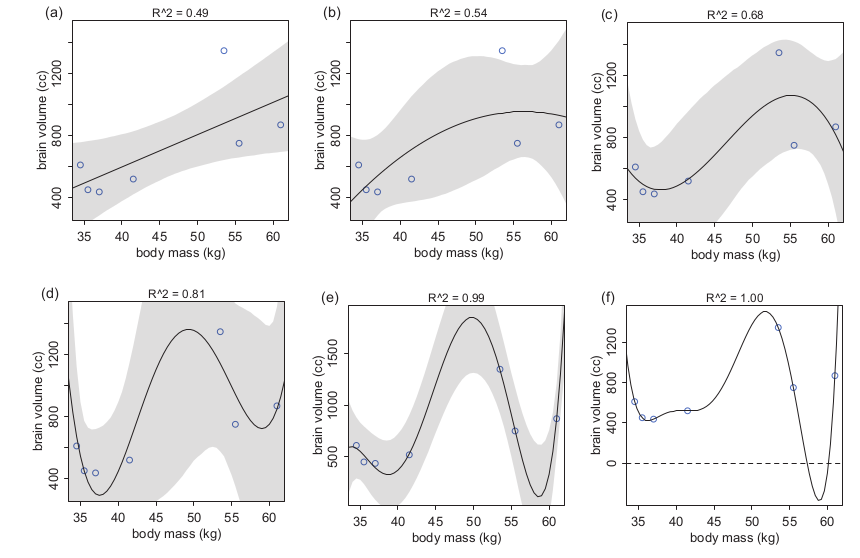
\includegraphics[scale=0.41]{pics/polyover.png}
\end{figure}

Polynomial linear models of increasing degree, fit to the hominin data. Each plot shows the predicted mean in black, with 89\% interval of the mean shaded. $R^2$, is displayed above each plot. (a) First-degree polynomial. (b) Second-degree. (c) Third-degree. (d) Fourth-degree. (e) Fifth-degree. (f) Sixth-degree. Source: \cite{mcelreath2020statistical}. 

} 
\end{frame}




\begin{frame}{The problem with parameters}
\scriptsize{

\begin{itemize}

\item We can see from looking at the paths of the predicted means that the higher-degree polynomials are increasingly absurd. 

\item For example, \textbf{reg.ev.6} the most complex model makes a perfect fit, but the model is ridiculous. 

\item Notice that there is a gap in the body mass data, because there are no fossil
hominins with body mass between 55 kg and about 60 kg. 
\item In this region, the models has nothing to predict, so it pays no price for swinging around wildly in this interval.
\item The swing is so extreme that at around 58 kg, the model predicts a negative brain size!

\item The model pays no price (yet) for this absurdity, because there are no cases in the data with body mass near 58 kg.

\end{itemize}


} 
\end{frame}



\begin{frame}{The problem with parameters}
\scriptsize{

\begin{itemize}

\item Why does the sixth-degree polynomial fit perfectly? 
\item Because it has enough parameters to assign one to each point of data.

\item The model's equation for the mean has 7 parameters:

\begin{displaymath}
 y_i=\beta_{0}+\beta_{1}x_i +\beta_{2}x_i^2 +\beta_{3}x_i^3 +\beta_{4}x_i^4 ++\beta_{5}x_i^5+\beta_{6}x_i^6+\epsilon_i \quad \forall i
\end{displaymath}
and there are 7 species to predict brain sizes for.

\item So effectively, this model assigns a unique parameter to reiterate each observed brain size.
\item This is a general phenomenon: If you adopt a model family with enough parameters, you can fit the data exactly. 
\item But such a model will make rather absurd predictions for yet-to-be-observed cases.


\end{itemize}


} 
\end{frame}


\begin{frame}[fragile]{Too few parameters hurts, too}
\scriptsize{

\begin{itemize}
\item The overfit polynomial models manage to fit the data extremely well.

\item But they suffer for this within-sample accuracy by making nonsensical out-of-
sample predictions.

\item In contrast, underfitting produces models that are inaccurate both
within and out of sample.

\item For example, consider this model of brain volume:

\begin{displaymath}
 y_i=\beta_{0}+\epsilon_i \quad \forall i
\end{displaymath}

\item There are no predictor variables here, just the intercept $\beta_{0}$.

\item We can fit this model as follows:

\begin{verbatim}
> reg.ev.0 <- lm( brain ~ 1 , data=d )
> summary(reg.ev.0)$r.squared
[1] 0 
\end{verbatim}

\item The value of $R^2$ is 0.

\end{itemize}


} 
\end{frame}


\begin{frame}[fragile]{Too few parameters hurts, too}
\scriptsize{

\begin{itemize}


\item This model estimates the mean brain volume, ignoring body mass.


\begin{figure}[h!]
	\centering
	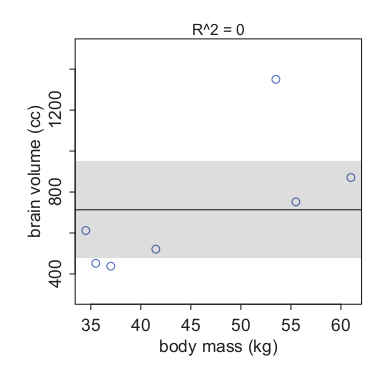
\includegraphics[scale=0.41]{pics/regconstant.png}
\end{figure}

\item As a result, the regression line is perfectly horizontal and poorly fits both smaller and larger brain volumes.

\item Such a model not only fails to describe the sample.

\item It would also do a poor job for new data

\end{itemize}


} 
\end{frame}


\begin{frame}{Roadmap}
\scriptsize{

\begin{itemize}
\item The first thing we need to navigate between overfitting and underfitting problems is a criterion of model performance.

\item We will see how information theory provides a useful criterion for model evaluation: the \textbf{out-of-sample deviance}.

\item Once we learn about this cretierion we will se how both regularization and information criteria help to improve and estimate the out-of-sample deviance of a model.

\item As usual, we will introduce these concepts with an example.

\end{itemize}


} 
\end{frame}

\begin{frame}{The Weatherperson}
\scriptsize{

\begin{itemize}
\item Suppose in a certain city, a certain weatherperson issues uncertain predictions for rain or shine on each day of the year.

\item The predictions are in the form of probabilities of rain. 

\item The currently employed weatherperson predicted these chances of rain over a 10-day sequence: 

\begin{figure}[h!]
	\centering
	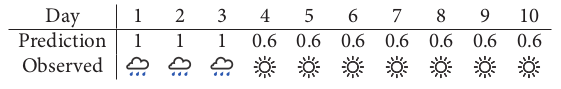
\includegraphics[scale=0.41]{pics/weather1.png}
\end{figure}


\item A newcomer rolls into town, and this newcomer boasts that he can best the current weatherperson, by always predicting sunshine. 

\item Over the same 10 day period, the newcomer's record would be:

\begin{figure}[h!]
	\centering
	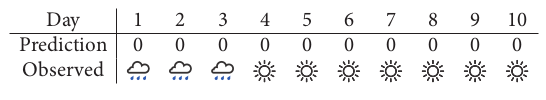
\includegraphics[scale=0.41]{pics/weather2.png}
\end{figure}


\end{itemize}


} 
\end{frame}


\begin{frame}{The Weatherperson}
\scriptsize{

\begin{itemize}
\item Define hit rate as the average chance of a correct prediction. 
\item So for the current weatherperson, she gets $3 \times 1 + 7 \times 0.4 = 5.8$ hits in 10 days, for a rate of $5.8/10 = 0.58$ correct predictions per day.
\item In contrast, the newcomer gets $3 \times 0 + 7 \times 1 = 7$, for $7/10 = 0.7$ hits per day. 
\item The newcomer wins.

\item Let's compare now the two predictions using another metric, the joint likelihood: $\prod f(y_i;\theta)$ for a frequentist model or $\prod f(y_i|\theta)$ for a Bayesian one.

\item The joint likelihood corresponds to the joint probability of correctly predicting the observed sequence.


\item To calculate it we must first compute the probability of a correct prediction for each day.

\item Then multiply all of these probabilities together to get the joint probability of correctly predicting the observed sequence. 



\end{itemize}


} 
\end{frame}

\begin{frame}{The Weatherperson}
\scriptsize{

\begin{itemize}
\item The probability for the current weather person is $1^3 \times 0.4^7 \approx 0.005$. 

\item For the newcomer, it's $0^3 \times 1^7 = 0$. 
\item So the newcomer has zero
probability of getting the sequence correct. 
\item This is because the newcomer's predictions never expect rain.
\item So even though the newcomer has a high average probability of being correct
(hit rate), he has a terrible joint probability (likelihood) of being correct.

\item And the joint likelihood is the measure we want. 

\item Because it is the unique measure that correctly counts up the relative number of ways each event (sequence of rain and shine) could happen.

\item In the statistics literature, this measure is sometimes called the
\textbf{log scoring rule}, because typically we compute the logarithm of the joint probability and report that.


\end{itemize}


} 
\end{frame}


\begin{frame}{Information and uncertainty}
\scriptsize{

\begin{itemize}
\item So we want to use the log probability of the data to
score the accuracy of competing models. 
\item The next problem is how to measure distance from
perfect prediction.
\item A perfect prediction would just report the true probabilities of rain on each day. 
\item So when either weatherperson provides a prediction that differs from the target, we can measure the distance of the prediction from the target.

\end{itemize}


} 
\end{frame}


\begin{frame}{Information and uncertainty}
\scriptsize{

\begin{itemize}

\item What kind of distance should we adopt?

\item Getting to the answer depends upon appreciating what an accuracy metric needs to do.

\item It should appreciate that some targets are just easier to hit than other targets. 
\item For example, suppose we extend the weather forecast into the winter. Now there are three types of days:
rain, sun, and snow.
\item Now there are three ways to be wrong, instead of just two.
\item This has to be reflected in any reasonable measure of distance from the target, because by adding another type of event, the target has gotten harder to hit.

\item Before presenting a distance metric that satisfies the properties described above, we must introduce some concepts from information theory.

\end{itemize}


} 
\end{frame}

\begin{frame}{Regularization}
\scriptsize{

\begin{itemize}
\item Blabla
\end{itemize}


} 
\end{frame}

\begin{frame}{Information criteria}
\scriptsize{

\begin{itemize}
\item Blabla
\end{itemize}


} 
\end{frame}


\begin{frame}{Using information criteria}
\scriptsize{

\begin{itemize}
\item Blabla
\end{itemize}


} 
\end{frame}




\begin{frame}{Conclusions}
\scriptsize{

\begin{itemize}
\item Blabla
\end{itemize}


} 
\end{frame}


%%%%%%%%%%%%%%%%%%%%%%%%%%%
\begin{frame}[allowframebreaks]\scriptsize
\frametitle{References}
\bibliography{bio}
\bibliographystyle{apalike}
%\bibliographystyle{flexbib}
\end{frame}  









%%%%%%%%%%%%%%%%%%%%%%%%%%%

\end{document}
